\section{Metodología}
En este trabajo se propone un método que permite evaluar la precisión de un modelo con la técnica de regresión lineal; y se basa en implementar diversos esquemas de remuestreos y estimar la precisión, a través de intervalos de confianza Bootstrap para el coeficiente de determinación $R^2$, del modelo de regresión entre los valores reales y predichos del modelo que se desea evaluar.\\

Se consideraron cuatro escenarios posibles con respecto al cumplimiento o no de los supuestos de normalidad y de varianza constante para un modelo a evaluar: NVC, NNVC, NVD y NNVD. Para estimar la distribución del coeficiente de determinación $R^2$, se implementan ocho esquemas de remuestreos: el Bootstrap Robusto Simple; el Wild Bootstrap robusto propuesto en \textcite{rana-2012} con los tres esquemas de remuestreo propuestos por\textcite{wu-1986}, y los dos esquemas propuestos por \textcite{wu-1986}; el Bootstrap de residuales balanceado y el Bootstrap pareado balanceado. Se proponen los intervalos percentiles y el Bca para estimar $R^2$ y para su cómputo se utilizan $B=1,000$ remuestras para cada uno de los esquemas Bootstrap.\\ 

Se realizó un estudio de simulación para comparar las eficacias de los intervalos de confianza para los diferentes esquemas Bootstrap, tamaños de muestra y tipo de modelo; se simularon y evaluaron un total de 120,000 modelos, de los cuales 60,000 modelos fueron Exactos-Precisos (EP) y 60,000 fueron Exactos-Imprecisos (EI); para cada uno de los modelos se identificaron las $R^2$ de origen utilizadas para su simulación. Se simularon modelos de tamaños $n=10, 15, 20, 25, 30, 35$ para cada uno de los supuestos y tipo de modelo.\\  

Se consideraron tres criterios para determinar las eficacias de los intervalos para cada esquema Bootstrap, el primer criterio determina la eficacia como el porcentaje de las veces en que el intervalo contiene a la $R^2$ de origen para los modelos EP simulados; y viceversa, para los modelos IP la eficacia se determinó como el porcentaje de las veces en que el intervalo de confianza no contiene a la $R^2$ de origen. El segundo criterio determina la eficacia como el porcentaje de las veces en que ambos intervalos contienen de manera simultánea a la $R^2$ de origen para los modelos EP y de manera viceversa cuando ambos no la contienen para los modelos EI; y el tercer criterio determina la eficacia como el porcentaje de las veces en que uno de los intervalos es más estrecho que el otro cuando ambos intervalos contienen simultáneamente la $R^2$ de origen para los modelos EP y de manera viceversa uno de los intervalos es más estrecho que el otro cuando ambos no la contienen simultáneamente para los modelos EI.\\

Se analizaron las eficacias de los intervalos para cada tipo de supuesto a través de un ANOVA factorial para identificar diferencias significativas entre los tipos de intervalos, tipos de esquemas y tamaños de muestra; complementándolo con pruebas de Tukey. De acuerdo al análisis de los resultados se consideró una propuesta final para la evaluación de la precisión de un modelo, la cual se implementó en el lenguaje R \parencite{R-2024}; y se ilustra con dos modelos correspondientes a casos reales que se ajustaron a cada uno los diferentes escenarios.




\subsection{Una Propuesta para Evaluar la Precisión de un Modelo}

En esta propuesta para evaluar la precisión de un modelo se considera: el conocimiento del tipo de caso de esté ante los cuatro escenarios posibles bajo el cumplimiento de los supuestos de normalidad y/o varianza contante, los predichos $(z)$, los observados $(y)$ para generar muestras Bootstrap del coeficiente de determinación $R^{2}$. Se propone construir intervalos de confianza con el método Percentil y BCa a través de las muestras obtenidas, por ocho esquemas Bootstrap. \\ 

\subsubsection{Estimadores y Esquemas Bootstrap}

Se debe considerar tres tipos de casos bajo el cumplimiento de los supuestos de normalidad y/o varianza contante:

\begin{description}
	\item[] Caso - 1 NVC
	\item[] Caso - 2 NNVC
	\item[] Caso - 3 NVD \& NNVD
\end{description}


Es necesario construir los intervalos de confianza con los métodos: Percentil y BCa para la $R^{2}$. Dado el desconocimiento de la función de distribución del coeficiente de determinación, se propone el uso de los esquemas Bootstrap propuestos en \textcite{rana-2012} e implementados en \textcite{zacarias-2023}, al igual de los dos esquemas Bootstrap implementados en \textcite{balam-2012}. Dependiendo el caso a evaluar se utiliza los estimadores de mínimos cuadrados o el MM-estimador robusto.\\


\textit{Estimador de mínimos cuadrados para el Caso 1- NVC.}. En este caso se propone utilizar los estimadores al correr una regresión simple, junto a los residuales y los valores ajustados $\hat{y}$ obtenido por la regresión.\\


\textit{MM-estimador para el Caso 2- NVC y  Caso - 3 NVD \& NNVD}. En ambos casos se propone utilizar el MM-estimador con regresión robusta junto con los residuales robustos y los valores ajustados $\hat{y}$ robustos obtenidos por la regresión. Para el Caso 2- NVC, los residuales robustos se utilizaran sin ponderar y para el  Caso - 3 NVD \& NNVD los residuales robustos se ponderaran.  \\



\textit{Bootstrap robusto y Bootstrap de Residuales Balanceados para todos los casos}. Para todos los casos se propone utilizar siete esquemas Bootstrap a los residuales dependiendo sus caso, los siguientes esquemas robustos: los tres de Wu (\textit{Algoritmo 3.5.1.1, Algoritmo 3.5.1.2 y Algoritmo 3.5.1.3}), los dos de Liu (\textit{Algoritmo 3.5.1.4 y Algoritmo 3.5.1.5}) y el Bootstrap Robusto Simple (\textit{Algoritmo 3.4.2 y Algoritmo 3.4.7}) . Adicionalmente, se propone implementar justo a los seis esquemas robustos, el Bootstrap de Residuales Balanceados (\textit{Algoritmo 3.4.5}). \\


\textit{Bootstrap Pareado Balanceado para todos los casos}. El Bootstrap Pareado Balanceado (\textit{Algoritmo 3.4.6}) al aplicar el remuestreo sobre una muestra pareada de las observaciones con su respectiva predicha y no depender de los estimadores al uno utilizar los residuales, se implementa sin importar el tipo de caso, con las $z$ y $y$ proporcionadas.\\

Este proceso que permite desarrollar los esquemas Bootstrap dependiendo del caso del modelo se encuentra descrito en la Figura ~\ref{fig:AlgDifEsqBoots}

 

\begin{figure}[ht!]
	\centering 
	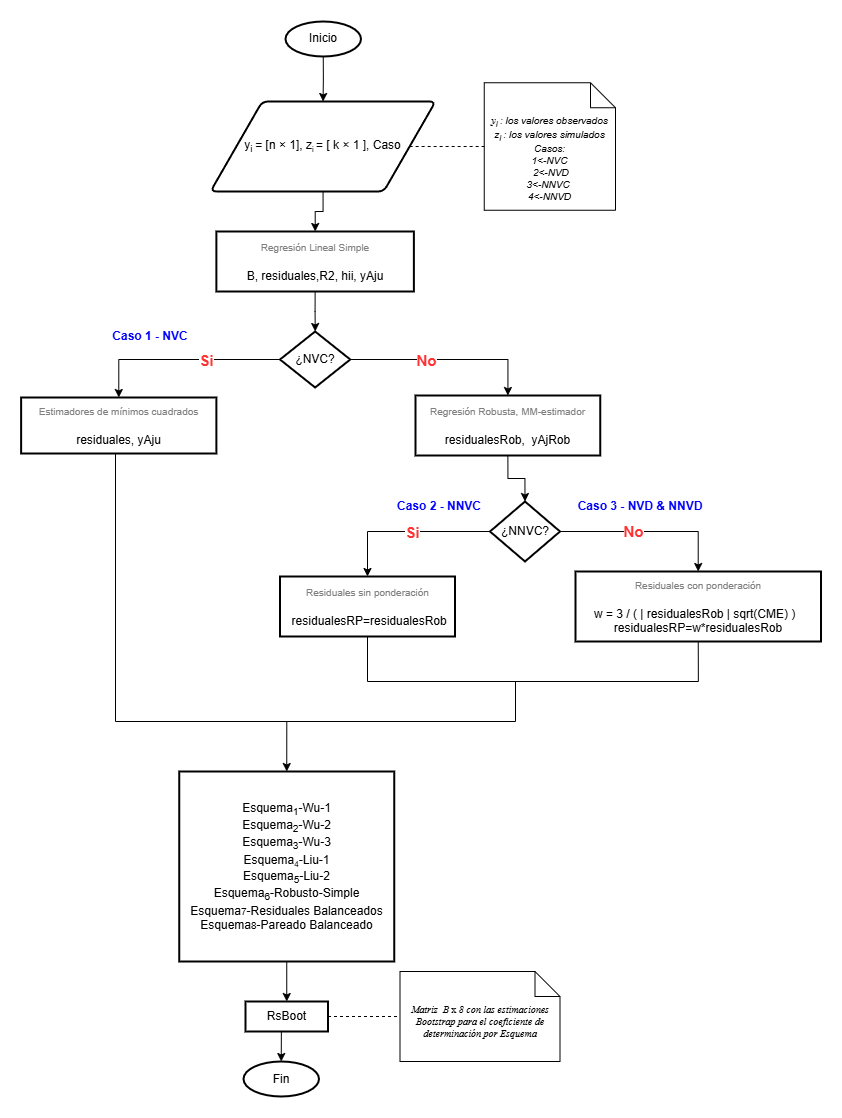
\includegraphics[width=0.4\linewidth]{img/metodologia_v6.png} 
	\caption{Algoritmo para los diferentes esquemas Bootstrap.}
	\label{fig:AlgDifEsqBoots}
\end{figure}
\FloatBarrier

\subsubsection{Intervalos de Confianza para la $R^{2}$}

Para evaluar la precisión del modelo se propone utilizar los intervalos de confianza Percentil y BCa para cada una de las muestras de $R^{2}s$ obtenidas en el procedimiento anterior por esquema Bootstrap. Debido a que las muestra Bootstrap de $R^{2}s$ ya se tiene, para el computo del I.C Percentil el \textit{Algoritmo 3.6.1} se comienza desde el paso 3. Y para el computó del I.C BCa se realiza el paso 1 del \textit{Algoritmo 3.6.2} en el cual se obtiene la estimación de la $R^{2}$ a partir de los datos originales del modelo, y se omiten los pasos 2 y 3 de dicho algoritmo ya que como en el caso anterior la muestra Bootstrap de $R^{2}s$ ya se tiene.\\



A continuación se describe el algoritmo para evaluar la precisión de un modelo construyendo intervalos de confianza para cada esquema Bootstrap:\\


\textbf{Algoritmo 4.1.2.1 - Evaluación la Precisión de un Modelo}

\begin{enumerate}
	
	\item Llamar la función y aplicar el algoritmo con los esquemas Bootstrap para generar la matriz \( \mathbf{RsBoot} \) de orden \( b \times k \), donde:
	\begin{itemize}
		\item \( b \) es el número de remuestras generadas (\( \hat{R}^{2*}_{1}, \hat{R}^{2*}_{2}, \dots, \hat{R}^{2*}_{b} \)).
		\item \( k \) es el número de esquemas Bootstrap considerados (\( k = 8 \)).
	\end{itemize}
	
	\item Para cada columna \( k \) (\( k = 1, 2, \dots, 8 \)) en la matriz de remuestras \( RsBoot \):
	\begin{itemize}
		\item Construir el intervalo de confianza Percentil \( [LI_{P_k}, LS_{P_k}] \) utilizando el \textit{Algoritmo 3.6.1} modificado previamente.
		\item Construir el intervalo de confianza BCa \( [LI_{BCa_k}, LS_{BCa_k}] \) utilizando el \textit{Algoritmo 3.6.2} modificado previamente.
	\end{itemize}
\end{enumerate}





	 
\subsection{Estudio de Simulación para la Evaluación de la Propuesta}

Para evaluar la eficacia de los intervalos de confianza con los diferentes esquemas Bootstrap, realizo un estudio de simulación donde se simularon modelos con la propuesta de \textcite{febles-2014} y las mejoras establecidas en \textcite{zacarias-2023}; para ello los modelos simulados se consideraron los siguientes factores: Precisión (EP, EI) con los supuesto (NVC, NVD, NNVC, NNVD). Tanto para los modelos EP y EI se utilizarán números aleatorios para $R^{2}$.


\subsubsection{Simulación de los Modelos}
Para la simulación de los modelos se utilizaron los simuladores $ModNVC()$, $ModNNVC()$, $ModNNVD()$ y$ ModNVD()$ descritos en la sección 3.7. Para este trabajo se simularon modelos de tipo EP y EI, por lo que se consideraron valores a priori fijos para el intercepto y la pendiente con b0=0 y b1=1; lo cual implicó que para el uso de los simuladores solo se tuviera que especificar tres argumentos: n, R2 y muz.\\

Los modelos se simularon para tamaños de muestra n=10, 15, 20, 25, 30, 35; para los valores hipotéticos de R2, se seleccionaron números aleatorios en el intervalo (0.8, 0.99) para los modelos EP y números aleatorios en el intervalo (0.1, 0.3) para los modelos EI, en ambos casos los números se redondearon a cuatro decimales. Para la especificación de muz se consideraron número aleatorios en el intervalo (5,100).\\
 

\subsubsection{Generación y Respaldo de los Modelos Simulados}

Para la simulación y el respaldo de todos los modelos utilizados para evaluar la propuesta de este trabajo, se desarrolló la función $SimMod(N,n,r,TipoPres,TipoSupues)$; la cual tiene como argumentos el número de modelos que se desean simular (N); el tamaño de la muestra (n); el número de réplicas para cada modelo (r);  la precisión deseada (TipoPres; 1: Preciso, 2:Impreciso); y tipo de supuesto que debe cumplir el modelo simulado (TipoSupues; 1:NVC, 2:NVD, 3:NNVC, 4:NNVD). Para todos los tipos de modelos simulados se consideraron r=5 réplicas para N=500 modelos; de tal forma que, para un tamaño de muestra fijo, un tipo de precisión fijo y un tipo de supuesto fijo se simularon 2,500 modelos; por lo que en total se simularon y respaldaron $120,000 modelos$ (2500x6x2x4), la mitad fueron modelos EP y la otra mitad modelos EI.
La función SimEP() ejecuta para cada réplica, el simulador correspondiente ($ModNVC()$, $ModNVD()$,$ ModNNVC()$,$ ModNNVD()$)  N veces para la simulación de los modelos correspondientes a cada tipo de supuesto. Al final, la función $SimEP()$ guarda los modelos simulados por cada tamaño de muestra, tipo de precisión y tipo de supuesto en una matriz de tamaño $rn \times 2N$ y también guarda en otra matriz de tamaño $r \times N$ a las $R^2$ correspondientes a cada uno de los modelos simulados, en total se respaldaron 48 matrices que contienen los 120,000 modelos y 48 matrices que contienen las $R^2$ correspondiente a cada modelo simulado. Las matrices se utilizaron para determinar las eficacias de los métodos Bootstrap propuestos para la medición de la precisión de un modelo. Para más detalle sobre la función $SimEP()$ ver Anexo C.\\

Revisar el Anexo C, se muestran las ejecuciones realizadas a la función $SimEP ()$ para la simulación y respaldo de los 120,000 modelos utilizados. \\


\subsubsection{Evaluación de la Precisión de los Modelos}

Después de simular los modelos hipotéticos EP e EI con los cuatro supuestos, se construyó la función $ProcesarModels()$ y la función $EvalPrecisionModel()$ para evaluar la precisión, donde para la primera función $ProcesarModels$, recibe los siguientes argumentos: $"archivos_encontrados"$ que representa dos archivos: la matriz de $rn \times 2N$ con los modelos y la matriz de $r \times N$ con las $R^2$ respectivas; $"caso"$ indica el tipo de escenario de los modelos, con 1 como Normalidad- Homocedasticidad, 2 como Normalidad-Heterocedasticidad, 3 como No normalidad-Homocedasticidad y 4 como No normalidad-Heterocedasticidad; $"replicas"$ como el número de replicas del estudio; $"nivConfianza"$ como el nivel de confianza para el I.C. para la $R^2$; $"N"$ como el tamaño de muestra de los modelos; $"MODELO"$ para indicar si es preciso o impreciso y $"CASO"$ como una etiqueta del tipo de supuesto($"NVC","NVD","NNVC","NNVD"$).\\


La función al procesar ambas matrices (modelos y sus $R^2$s) por replica, recupera uno por uno los modelos y se le pasa a la función $EvalPrecisionModel()$ que implementa el \textit{Algoritmo 4.1.2.1} con $B=1,000$ remuestras Bootstrap por cada uno de los ocho tipos de remuestreos y calcula los I.C., el cual recibe los parámetros de $"data"$ como el vector $ z \times y $ con los predichos y las observaciones respectivamente del modelo;  $"alpha"$ como el nivel de significancia; $" nivConfianza" $, el nivel de confianza y el $"caso"$, que retorna una lista de ocho matrices de tamaño $2 \times 2$, donde cada uno matriz contiene los I.C. Percentil e I.C BCa para el coeficiente de determinación calculado por cada esquema para el modelo.\\


\subsubsection{Determinación de la Eficacia de los Intervalos y Esquemas}

Al obtener la lista con los I.C. para la $R^2$ del modelo, estos se procesan por esquema y  se realizan las evaluaciones para determinar las eficacias, pero antes, deber cumplir el criterio de que los intervalos con el esquema hayan sido calculados, es decir, son valores válidos, para considerarlo un modelo eficaz con el esquema. La eficiencia se determinó como el porcentaje de veces que los intervalos contienen a la \( R^2 \) de origen empleada para simular el modelo. Adicionalmente, para evaluar cuál de los dos intervalos es más eficaz, se consideraron dos escenarios: si solo uno de los intervalos logró contener la \( R^2 \), se consideró ganador por defecto y la eficacia se calculó como el porcentaje de veces en que solo uno de los intervalos incluyó la \( R^2 \); en caso de empate, es decir, cuando ambos intervalos contuvieron la \( R^2 \), se consideró más eficiente el intervalo con menor amplitud, ya que proporciona una estimación más precisa. La eficacia en este caso se calculó como el porcentaje de veces que ambos intervalos incluyeron la \( R^2 \), pero uno de ellos fue más estrecho.\\

La eficacia de los esquema Bootstrap, se determinó como el porcentaje de veces que logra que ambos intervalos contengan a la \( R^2 \) de origen con respecto a los modelos evaluados.\\

Los resultado de las eficacias se respaldan por supuesto y tipo de modelo, y sus replicas con dos tablas: para la eficacia de los intervalos se guarda el numero de replica, el identificador del esquema utilizado, el numero de modelos dados por la replica, el número de modelos eficaces en la replica que cumplieron la condición de construir ambos intervalos con valores válidos, la frecuencia de en que el I.C Percentil es eficiente, la frecuencia de en que el I.C BCa es eficiente, la frecuencia en la que el I.C Percentil fue el ganador por defecto, la frecuencia en la que el I.C BCa fue el ganador por defecto, la frecuencia en la que el I.C. Percentil fue mejor que el I.C. BCa al ambos contenerlo y la frecuencia en la que el I.C. BCa fue mejor que el I.C. Percentil al ambos contenerlo. Para la eficacia del esquema la tabla almacena por replica el número de veces en la que el esquema logro hacer que sus I.C. contuvieran a la \( R^2 \) de origen. \\



\subsection{Análisis estadísticos}
Para cada supuesto (NVC, NNVC, NVD, NNVD) se utilizó ANOVA en un arreglo factorial de tres factores seguido de la comparación múltiple de Tukey \parencite{montgomery-2017}, para determinar el comportamiento de la eficacia de dos ICB en la evaluación de la precisión, bajo ocho esquemas de remuestreo, seis tamaños de muestra y dos tipos de modelo. Cabe señalar que, en cuatro de los ocho análisis de varianza realizados se eliminaron valores atípicos para el logro del cumplimiento de los supuestos del ANOVA.
Las pruebas estadísticas se consideraron significativas cuando  y se utilizó el paquete estadístico STATGRAPHICS Centurion 19 \parencite{statgraphics-2024} .




